\documentclass[letterpaper, 12pt]{article}

\usepackage[utf8]{inputenc}
\usepackage[english, spanish]{babel}
% \usepackage{newtxtext}
\usepackage{fullpage}
\usepackage{graphicx}
\usepackage{amsmath}
\usepackage{enumitem}
\usepackage{chngcntr}
\usepackage{setspace}
\usepackage{url}
\usepackage{csquotes}
\usepackage{float}
\usepackage{verbatim}
\usepackage{tabularx}
\usepackage{amsmath}
\usepackage{caption}
\usepackage{bm}
\usepackage{colortbl}
\usepackage{xcolor}
\usepackage{multicol}
\usepackage{wrapfig}
\usepackage{multirow}

% \usepackage{hyperref}

\counterwithin{figure}{section}
\renewcommand{\thesection}{\arabic{section}}
\renewcommand{\thesubsection}{\thesection.\arabic{subsection}}
\renewcommand{\baselinestretch}{1.5}

\usepackage[style=apa, maxnames=6, minnames=3, backend=biber, parentracker=true, sorting=none]{biblatex}
\DefineBibliographyStrings{english}{%chktex-file 1 chktex-file 6
      andothers = {\em et\addabbrvspace al\adddot}
}
\addbibresource{./Bibliography/bibliography.bib}

\usepackage{array}

\setlength{\parskip}{0pt}

\raggedbottom{}

\newcommand{\bolditalic}[1]{\textbf{\textit{#1}}}

\begin{document}

\begin{titlepage}
      \centering
      
\includegraphics[width=0.3\textwidth]{Images/logo_utb.png}\par\vspace{1cm}
      {\scshape\LARGE Universidad Tecnológica de Bolívar \par}
      \vspace{1cm}

      {\scshape\Large Materiales \par}
      \vspace{1cm}

      \slshape {\Large \bfseries{}COMPUESTOS DE MATRIZ METALICA EN LA INDUSTRIA DE DEFENSA\\}
      \vspace{4cm}

      \slshape {\itshape{}Daniela Patricia Hollmann Guarin, T00078865 \\}
      \slshape {\itshape{} Nathaly Sofia Castillo Moreno, T00078553 \\}
      \vfill
      Revisado Por \\
      Darling Perea Cabarcas\\
      {\large \today\par}
\end{titlepage}

\nocite{*}

% chktex-file 8
% chktex-file 44
% chktex-file 24

\section{Resumen}

El presente trabajo analiza los compuestos de matriz metálica (CMM), destacando
su combinación de matriz metálica y refuerzos cerámicos o de carbono para
lograr propiedades superiores como alta resistencia, rigidez, ligereza y
resistencia a la corrosión. Se enfocan en su uso en defensa, especialmente en
blindajes, componentes estructurales, motores y sistemas de armamento. También
aborda los métodos avanzados de fabricación y los desafíos asociados, como los
altos costos y la distribución uniforme de refuerzos, resaltando su potencial
estratégico en aplicaciones extremas y su prometedor futuro en otras
industrias.

\newpage

\tableofcontents
\newpage

\section{Introduccion}

Los materiales compuestos de matriz metálica (MMC) constituyen una categoría de
materiales avanzados que se obtienen mediante la combinación de dos o más
componentes con propiedades diferentes, lo que resulta en características
singulares que no se presentan en los materiales individuales. La sinergia
entre la matriz metálica y el refuerzo mejora propiedades como la resistencia,
la rigidez y la conductividad térmica y eléctrica. Estas cualidades hacen que
los MMC sean muy valorados en diversas aplicaciones de ingeniería.

Las matrices metálicas utilizadas en los compuestos de matriz metálica (CMM)
son esenciales como el componente continuo que distribuye las cargas aplicadas,
aportando propiedades específicas que mejoran las capacidades del material
compuesto. Los materiales más comunes incluyen aluminio, magnesio, cobre y
titanio, cada uno con ventajas particulares que los hacen adecuados para
diferentes aplicaciones. El aluminio (Al), por ejemplo, es ligero, resistente a
la corrosión y un excelente conductor térmico, características que lo
posicionan como una opción ideal para blindajes y componentes estructurales en
aeronaves militares.

Por otro lado, el titanio (Ti) se destaca por su alta resistencia específica y
su capacidad de soportar temperaturas extremas, lo que lo hace indispensable en
motores de aviones y estructuras de misiles y cohetes. El magnesio (Mg), siendo
más ligero que el aluminio, ofrece una alta relación rigidez/peso, aunque
presenta menor resistencia a la corrosión; por ello, se utiliza frecuentemente
en componentes de drones y equipos móviles donde la ligereza es prioritaria.
Finalmente, el cobre (Cu) sobresale por su excelente capacidad de conducción
térmica y eléctrica, siendo una opción valiosa en aplicaciones donde estas
propiedades son cruciales.

La selección de la matriz metálica adecuada depende directamente de las
necesidades específicas del diseño y las condiciones a las que estará sometido
el compuesto, lo que resalta la versatilidad de los CMM en diversos contextos,
especialmente en la industria de defensa. Los refuerzos en los compuestos de
matriz metálica (CMM) son fundamentales para proporcionar las propiedades de
rigidez, resistencia y durabilidad necesarias en aplicaciones exigentes. Estos
pueden presentarse en diferentes formas, como fibras, partículas o whiskers
(bigotes), y su selección depende de los requisitos específicos del diseño y
las condiciones operativas.

\subsection{Fibras continuas}

\begin{itemize}
      \item Materiales comunes: carbono, boro y cerámicas como el carburo de silicio (SiC)
      \item Ventajas: ofrecen una alta resistencia a la tracción y rigidez, siendo ideales
            para aplicaciones donde se requieren estructuras livianas y resistentes.
\end{itemize}

\subsection{Partículas}

\begin{itemize}
      \item Ejemplos: carburo de boro ($B_{4}C$) y óxido de aluminio ($Al_{2}O_{3}$).
      \item Aplicaciones: mejoran la resistencia al desgaste y la estabilidad frente a
            choques térmicos, lo que las hace adecuadas para armaduras y componentes
            sometidos a altas tensiones mecánicas.

\end{itemize}

\subsection{Whiskers}

\begin{itemize}
      \item Características: cristales cerámicos con estructuras regulares diseñadas para
            maximizar la resistencia mecánica y la rigidez.
      \item Usos: son ideales en aplicaciones que demandan propiedades mecánicas
            excepcionales en dimensiones pequeñas.

\end{itemize}

Entre los materiales de refuerzo más comunes, el carburo de silicio, el óxido
de aluminio y las fibras de carbono destacan por su alta resistencia a la
tracción, rigidez y capacidad para soportar el desgaste y los choques térmicos.
La elección del tipo de refuerzo y material adecuado depende de los requisitos
específicos de cada aplicación, maximizando así las propiedades del compuesto
final para satisfacer las demandas de sectores como la industria de defensa.

\begin{figure}[H]
      \begin{center}
            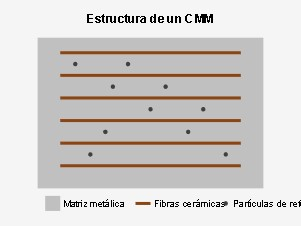
\includegraphics[width=.5\linewidth]{Images/Imagen1.jpg}
            \label{Diagrama donde se observa la composición interna de un CMM, se aprecia la matriz metálica y el refuerzo, como fibras de cerámica o partículas.}
      \end{center}
\end{figure}

Comparados con los compuestos de matriz polimérica (CMPP), los CMM son más
resistentes al calor y al desgaste, lo que los hace ideales para entornos
exigentes. La selección de los materiales que constituyen la matriz y el
refuerzo es fundamental para definir las propiedades finales de los compuestos
de matriz metálica (MMC). Estos son los componentes esenciales de los MMC.

\begin{figure}[H]
      \begin{center}
            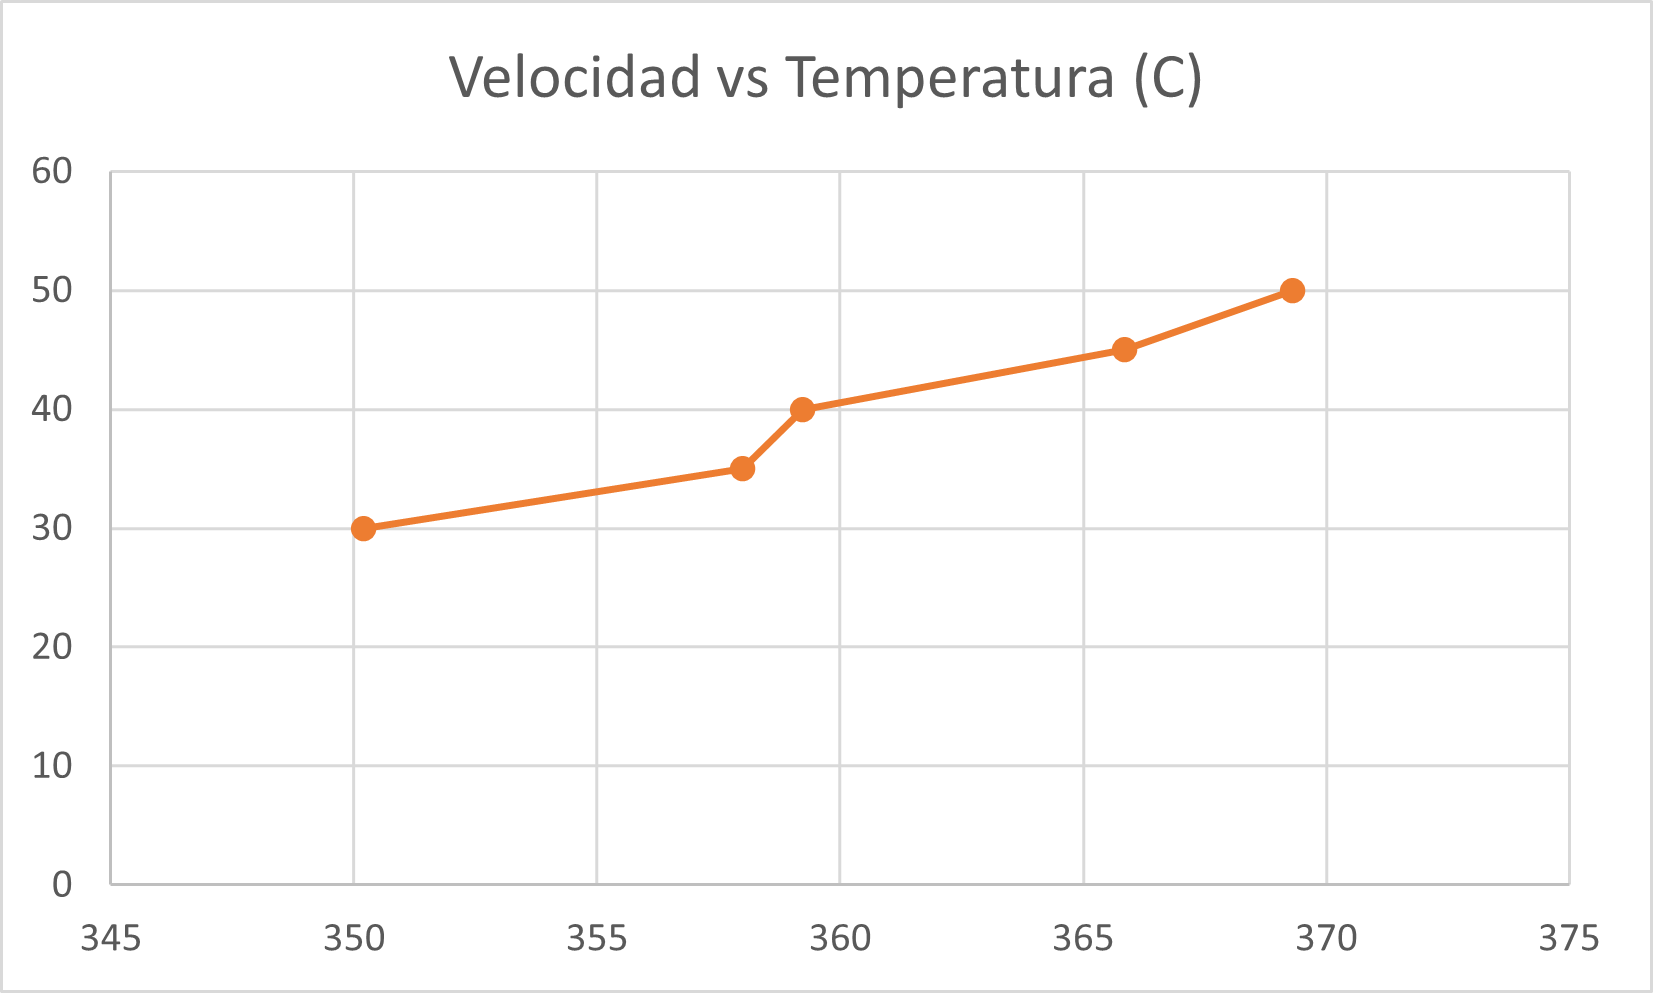
\includegraphics[width=.8\linewidth]{Images/Imagen2.png}
            \label{Gráfico comparativo entre CMM y materiales convencionales (como acero y aluminio) en términos de resistencia, peso y durabilidad.}
      \end{center}
\end{figure}

La característica más destacada de los MMC es su capacidad para fusionar la
ductilidad y tenacidad de los metales con la alta resistencia y rigidez de los
materiales de refuerzo. Esta combinación da lugar a materiales compuestos que
pueden satisfacer requisitos específicos, como los que se emplean en las
industrias aeroespacial y automotriz, donde se demandan altas prestaciones en
condiciones extremas.

\section{Evolución histórica}

Los compuestos de matriz metálica (CMM) comenzaron a investigarse en las
décadas de 1950 y 1960. Su desarrollo estuvo impulsado principalmente por las
necesidades aeroespaciales y de defensa, donde la alta resistencia, rigidez y
la reducción de peso son esenciales.

En este período, se utilizaban aleaciones ligeras como base, especialmente
aluminio y magnesio, con refuerzos cerámicos (carburo de silicio, óxido de
aluminio). En la década de 1970, los CMM comenzaron a usarse en componentes
estructurales y aplicaciones térmicas en misiles y aviones militares debido a
su alta resistencia específica y capacidad para operar en condiciones extremas.
En la Guerra Fría, la búsqueda de armas más ligeras y vehículos más rápidos
incentivó inversiones en investigación y desarrollo.

El desarrollo de procesos avanzados como la infiltración, la deposición en fase
gaseosa y la pulvimetalurgia permitió fabricar componentes más complejos y con
mejor calidad. Comenzaron a integrarse refuerzos como fibras continuas y
nanotubos para mejorar la ductilidad y el comportamiento ante impactos.

En el siglo XXI, el enfoque se desplazó hacia la fabricación aditiva y la
nanocomposición para optimizar el diseño y reducir los costos. Los sistemas de
armas modernos, drones y vehículos blindados han comenzado a incorporar CMM
para mejorar su rendimiento frente a balas, explosiones y altas temperaturas.

Los materiales compuestos han revolucionado múltiples industrias al ofrecer
soluciones personalizadas con propiedades optimizadas. En el ámbito de la
defensa, estos materiales desempeñan un papel clave gracias a características
como: Alta relación resistencia/peso, que reduce la carga en sistemas de
transporte militar. Resistencia al desgaste y a la fatiga, extendiendo la vida
útil de equipos críticos. Adaptabilidad para diseñar propiedades específicas
según las necesidades del campo de batalla.

El sector de defensa se posiciona como uno de los principales adoptantes de los
MMC, debido a las exigencias de alto rendimiento en situaciones de gran carga
mecánica, temperaturas elevadas y exposición a entornos adversos. La
combinación de ligereza, resistencia superior y durabilidad ante el desgaste es
crucial para diversas aplicaciones en defensa, que abarcan desde la producción
de vehículos blindados y aeronaves hasta el desarrollo de sistemas de munición
de alto rendimiento. Los compuestos de matriz metálica (MMC) son reconocidos
por sus propiedades excepcionales, lo que los convierte en recursos
especialmente valiosos en el ámbito de la defensa. A continuación, se presenta
un análisis detallado de sus principales características y de cómo estas
optimizan su aplicación en contextos militares.

\begin{enumerate}
      \item Alta resistencia mecánica
            \begin{itemize}
                  \item Análisis: Los materiales compuestos metálicos (MMC) ofrecen una resistencia
                        mecánica significativamente superior a la de los metales tradicionales, gracias
                        a la adición de refuerzos como partículas de carburo de silicio o fibras de
                        carbono. Esta notable resistencia les permite soportar cargas y fuerzas
                        intensas sin sufrir deformaciones.

                  \item Ventajas en defensa: Esta característica es esencial para el blindaje de
                        vehículos y los elementos estructurales de aeronaves y vehículos terrestres,
                        que deben ser capaces de resistir impactos y tensiones extremas en situaciones
                        de combate.
            \end{itemize}
      \item Rigidez elevada
            \begin{itemize}
                  \item Análisis: La incorporación de materiales cerámicos en su estructura permite a
                        los MMC alcanzar una rigidez considerablemente mayor en comparación con los
                        metales convencionales. Esto significa que los componentes elaborados con MMC
                        son menos propensos a la deformación elástica bajo carga.
                  \item Ventajas en defensa: Esta elevada rigidez garantiza que los MMC conserven su
                        integridad estructural y forma, lo cual es vital en aplicaciones que requieren
                        alta precisión y estabilidad, como en drones y aeronaves no tripuladas.
            \end{itemize}

      \item Ligereza y baja densidad

            \begin{itemize}
                  \item Análisis: Los MMC están formados por matrices metálicas de baja densidad, como
                        aluminio, magnesio o titanio. Esta característica, junto con su resistencia
                        mejorada, permite la creación de componentes que combinan ligereza y alta
                        resistencia.

                  \item Ventajas en defensa: La disminución del peso es crucial en vehículos y equipos
                        militares, ya que optimiza la maniobrabilidad y la eficiencia del consumo de
                        combustible. Los MMC contribuyen a reducir el peso de los componentes
                        estructurales, lo que a su vez mejora la velocidad y la capacidad de carga de
                        vehículos y aeronaves en aplicaciones militares.
            \end{itemize}

      \item Resistencia a altas temperaturas

            \begin{itemize}
                  \item       Análisis: Los materiales compuestos de matriz metálica (MMC) conservan sus
                        propiedades mecánicas a temperaturas elevadas debido a la estabilidad térmica
                        de los refuerzos cerámicos, lo que le confiere una menor tendencia a la
                        deformación en comparación con los metales convencionales.
                  \item Ventajas en defensa: En sistemas de propulsión de aeronaves y vehículos
                        militares que operan en condiciones de alta temperatura, los MMC proporcionan
                        un rendimiento fiable, asegurando la resistencia necesaria sin comprometer sus
                        características mecánicas en situaciones extremas.
            \end{itemize}

      \item Resistencia al desgaste y la corrosión

            \begin{itemize}
                  \item Análisis: Los MMC, especialmente aquellos reforzados con partículas cerámicas,
                        presentan una notable resistencia al desgaste y a la corrosión. Esta propiedad
                        prolonga considerablemente la vida útil de los componentes, incluso en entornos
                  \item Ventajas en defensa: Esta característica es esencial en vehículos militares y
                        sistemas de armamento que operan en condiciones adversas, como climas marinos o
                        desérticos, donde la corrosión y el desgaste pueden poner en riesgo la
                        funcionalidad y durabilidad del equipo. donde los metales tradicionales tienden
                        a corroerse o desgastarse rápidamente.
            \end{itemize}

      \item Absorción de energía

            \begin{itemize}
                  \item Análisis: Los MMC poseen una estructura que les permite absorber grandes
                        cantidades de energía antes de fracturarse, ya que los materiales cerámicos en
                        la matriz contribuyen a dispersar el impacto.

                  \item Ventajas en defensa: Esta capacidad es crucial para aplicaciones de protección
                        balística, ya que permite que el material absorba y disipe la energía de los
                        impactos sin romperse, lo que resulta fundamental en la fabricación de
                        blindajes tanto personales como para vehículos.
            \end{itemize}

      \item Conductividad térmica variable

            \begin{itemize}
                  \item Análisis: Los materiales compuestos metálicos (MMC) permiten la modificación de
                        su conductividad térmica a través de la elección de diversos refuerzos y
                        matrices, lo que facilita el diseño de materiales que gestionen el calor según
                        las necesidades específicas de cada aplicación, ya sea para disiparlo de manera
                        eficiente o para conservarlo.

                  \item Ventajas en defensa: Esta capacidad de ajustar la conductividad térmica resulta
                        fundamental en sistemas de armamento, dispositivos electrónicos y motores de
                        alto rendimiento, donde una adecuada gestión del calor es vital para prevenir
                        daños por sobrecalentamiento y asegurar un funcionamiento fiable y duradero del
                        equipo en condiciones extremas.
            \end{itemize}
\end{enumerate}

Los MMC integran características destacadas de resistencia, rigidez y
durabilidad, lo que los convierte en opciones ideales para aplicaciones en el
ámbito de la defensa. Su ligereza contribuye a la reducción del peso en
vehículos y aeronaves, mejorando así tanto la maniobrabilidad como la
eficiencia. Además, su resistencia a temperaturas extremas y al desgaste
garantiza un rendimiento constante en situaciones desafiantes, mientras que su
notable capacidad de absorción de energía los hace aptos para aplicaciones de
protección balística. Estas propiedades en conjunto ofrecen significativas
ventajas tácticas y logísticas en el contexto militar, optimizando la
seguridad, el rendimiento y la durabilidad de los sistemas de defensa.

\section{Procesamiento}

Los compuestos de matriz metálica (CMM) son materiales compuestos que consisten
en una matriz metálica reforzada con partículas o fibras. Su desarrollo ha sido
motivado por la necesidad de crear materiales que combinen la resistencia y
rigidez de los metales con las propiedades de los refuerzos cerámicos o de
carbono. Estas combinaciones ofrecen un rendimiento superior en comparación con
los metales puros, especialmente en aplicaciones que requieren alta resistencia
mecánica, estabilidad ante variaciones térmicas y un peso reducido.

\begin{figure}[H]
      \begin{center}
            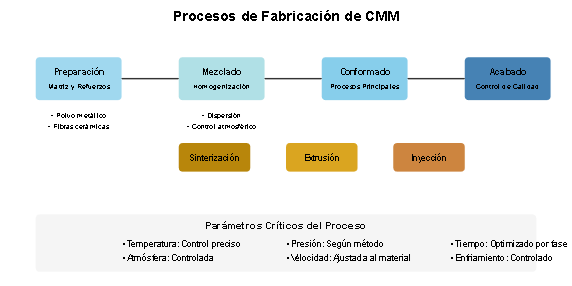
\includegraphics[width=\linewidth]{Images/Imagen3.png}
            \label{Diagrama de flujo de los procesos de fabricación de CMM, como la sinterización, la extrusión o la inyección, mostrando como se integran los refuerzos con la matriz metálica.}
      \end{center}
\end{figure}

\section{Métodos de Procesamiento de CMM}

\begin{itemize}
      \item Moldeo por compresión \\ En este procedimiento, los materiales en forma de
            polvo, tanto metálicos como de refuerzo, son sometidos a una compresión en un
            molde bajo condiciones de alta presión y temperatura. Esta técnica es eficaz
            para la obtención de componentes densos con una distribución uniforme de los
            refuerzos, siendo especialmente adecuada para la fabricación de piezas con
            geometrías complejas y excelentes propiedades mecánicas.
      \item Hipersinterización: \\ Este método representa una versión avanzada de la
            sinterización convencional, donde se aplican condiciones controladas de
            temperatura y tiempo para optimizar la unión entre la matriz metálica y el
            refuerzo cerámico. La hipersinterización incrementa la cohesión entre las
            diferentes fases, lo que se traduce en una mayor resistencia y durabilidad del
            material compuesto.

      \item Procesamiento por energía de alta intensidad (HEI): \\ Este enfoque utiliza
            fuentes de energía de alta intensidad, como plasma o microondas, para procesar
            y consolidar los materiales. Se utiliza principalmente en la producción de
            estructuras compuestas que incorporan materiales de refuerzo avanzados. La
            energía de alta intensidad facilita la fusión eficiente de la matriz metálica
            con el refuerzo, mejorando así las propiedades mecánicas y térmicas del
            producto final.

      \item Procesamiento por infiltración: \\ Este proceso consiste en la infiltración de
            la matriz metálica fundida en una preforma de refuerzo, ya sea cerámica o de
            fibra. Se emplea para crear compuestos con una distribución precisa de la
            matriz y el refuerzo, asegurando que las características del material final
            estén optimizadas según la aplicación específica.

      \item Corte láser de alta precisión: \\ Los componentes de CMM pueden ser elaborados
            mediante corte láser, lo que permite obtener formas exactas con tolerancias muy
            estrictas. Este proceso es ideal para piezas con geometrías complejas y
            proporciona un acabado superficial limpio, sin deformaciones térmicas
            significativas. La fabricación aditiva, comúnmente conocida como impresión 3D,
            representa una tecnología innovadora en la producción de compuestos de matriz
            metálica (CMM). Este método consiste en la deposición y consolidación de capas
            de material en polvo metálico y refuerzo, utilizando un láser o electrones para
            llevar a cabo el proceso. Gracias a esta técnica, es posible crear componentes
            con geometrías complejas que no podrían ser fabricados mediante métodos
            tradicionales. Asimismo, la impresión 3D permite el diseño de estructuras
            personalizadas que poseen una alta resistencia. Cada técnica de procesamiento
            asociada a esta tecnología ofrece beneficios particulares para la elaboración
            de CMM, lo que resulta en componentes con propiedades mecánicas, térmicas y
            estructurales superiores, aspectos esenciales para aplicaciones críticas en el
            sector de defensa.

\end{itemize}

\subsection{Compuestos de matriz metálica reforzados con fibras}

En estos compuestos, las fibras suelen ser de materiales como carbono, cerámica
(por ejemplo, carburo de silicio u óxido de aluminio) o metales. Las fibras
pueden estar dispuestas de manera orientada en una única dirección o
distribuidas de forma aleatoria, lo que permite optimizar las propiedades
mecánicas del compuesto según la dirección en la que se necesite el refuerzo.

\subsection{Compuestos de matriz metálica reforzados con partículas}

En lugar de utilizar fibras, se incorporan partículas cerámicas que se
dispersan en la matriz metálica. Estas partículas ayudan a mejorar
características como la dureza, la resistencia al desgaste y la conductividad
térmica. Ejemplos comunes de estas partículas son el carburo de boro, el
carburo de silicio y los óxidos de aluminio.

\subsection{Propiedades de los Compuestos de Matriz Metálica}

Los CMM presentan características superiores en comparación con los metales
convencionales, lo que los convierte en una opción muy atractiva para su
aplicación en la industria de defensa:

\begin{itemize}
      \item Alta resistencia mecánica: La inclusión de refuerzos cerámicos o de carbono
            incrementa tanto la resistencia a la tracción como a la compresión, mejorando
            notablemente las propiedades mecánicas de la matriz metálica.
      \item Peso reducido: Al utilizar materiales como el carbono o la cerámica en lugar de
            metales pesados, los CMM son más ligeros que los metales tradicionales, lo que
            los hace más eficientes en aplicaciones donde la reducción de peso es
            fundamental.
      \item Resistencia al desgaste y a la abrasión: Las partículas cerámicas o las fibras
            refuerzan la resistencia al desgaste y a la abrasión, características
            esenciales para componentes que operan en condiciones extremas, como en partes
            móviles de vehículos militares o sistemas de armamento.
      \item Alta conductividad térmica: Algunos CMM pueden ser diseñados para optimizar la
            conducción del calor, lo que los hace útiles en aplicaciones de alto
            rendimiento que funcionan a temperaturas extremas, como en sistemas de
            propulsión o motores.
      \item Resistencia a la corrosión: La notable resistencia a la corrosión que presentan
            muchos CMM los convierte en una opción ideal para entornos agresivos, como
            condiciones marinas o en contacto con productos químicos corrosivos.

\end{itemize}

\section{Aplicaciones de los CMM en la Industria de Defensa}

\begin{itemize}
      \item Blindaje y protección \\ Los compuestos de matriz metálica se emplean en la
            fabricación de blindaje balístico y armaduras para vehículos blindados,
            aeronaves y embarcaciones. Su combinación de alta resistencia al impacto y baja
            densidad los convierte en una opción ideal para aplicaciones que requieren una
            protección significativa sin incrementar el peso. Asimismo, los CMM se utilizan
            en la producción de placas y estructuras de blindaje para vehículos militares y
            protección personal, mejorando la resistencia sin comprometer la movilidad.

      \item Componentes de aeronaves y misiles \\ Dado que los CMM son capaces de soportar
            altas temperaturas y tensiones mecánicas extremas, son particularmente
            adecuados para la fabricación de motores de aeronaves y sistemas de propulsión.
            También se utilizan en la construcción de partes críticas de misiles, como las
            aletas, que deben ser ligeras, pero extremadamente robustas. En el sector
            aeroespacial, los CMM ayudan a reducir el peso total de las aeronaves, lo que a
            su vez mejora la eficiencia del combustible y optimiza el rendimiento.

      \item Sistemas de armamento: \\ Los CMM son perfectos para la fabricación de
            componentes de sistemas de armas de precisión, como cañones, rifles y
            proyectiles, gracias a su alta resistencia al desgaste y rigidez. Estos
            materiales prolongan la vida útil de los componentes, asegurando un
            funcionamiento más duradero en condiciones de uso extremas.

      \item Sistemas de propulsión y motores: \\ En motores y turbinas, los CMM se utilizan
            para fabricar componentes que operan bajo condiciones de altas temperaturas y
            presiones, como las palas de turbina y las cámaras de combustión. Estos
            materiales son capaces de resistir el estrés térmico y mecánico extremo,
            garantizando un rendimiento constante y fiable en aplicaciones críticas.

      \item Electrónica y comunicaciones:\\ En el ámbito de la electrónica, los CMM se
            utilizan en sistemas de radar, satélites y comunicaciones, donde su capacidad
            para conducir el calor y su resistencia al desgaste son fundamentales.
\end{itemize}

\section{Desafíos y limitaciones}

\begin{itemize}
      \item Costos de fabricación: Los CMM son significativamente más costosos que las
            aleaciones tradicionales debido al proceso de fabricación complejo y a los
            materiales de refuerzo. Los métodos avanzados, como la fabricación aditiva, aún
            no están completamente optimizados para una producción en masa rentable.
      \item Procesabilidad: Dificultades para lograr una distribución uniforme del refuerzo
            en la matriz metálica, lo que puede generar puntos débiles y reducir la
            fiabilidad del material. La unión entre matriz y refuerzo sigue siendo un área
            problemática, ya que la incompatibilidad química y térmica puede ocasionar
            fallas prematuras.
      \item Comportamiento bajo carga dinámica: Aunque son resistentes, algunos CMM tienen
            una menor ductilidad y tolerancia al daño en comparación con otros materiales
            metálicos, lo que puede ser una limitación en situaciones de impacto extremo.
      \item Fatiga y fractura: Los CMM pueden ser más susceptibles a la propagación de
            grietas debido a las tensiones acumuladas entre la matriz y los refuerzos,
            especialmente en ambientes de alta presión y temperatura.
      \item Compatibilidad ambiental: La interacción con entornos corrosivos o abrasivos,
            como agua salada o atmósferas con altas temperaturas, plantea desafíos para
            garantizar una larga vida útil en aplicaciones militares.
      \item Limitaciones en diseño: Los CMM a menudo carecen de maleabilidad, lo que
            restringe las formas y diseños posibles, especialmente para aplicaciones
            complejas en defensa.

\end{itemize}

Los compuestos de matriz metálica (CMM) desempeñan un papel crucial en la
industria de defensa, gracias a sus destacadas propiedades, que incluyen una
gran resistencia, ligereza, durabilidad ante el desgaste y estabilidad térmica.
Estas cualidades hacen que los CMM sean utilizados como opciones o adiciones a
materiales tradicionales en sistemas y equipos fundamentales, lo que optimiza
su rendimiento y confiabilidad en condiciones de alta exigencia. Como se
mencionó anteriormente algunas de las aplicaciones más relevantes de los CMM en
el ámbito de la defensa son:

El blindaje balístico y las armaduras son fundamentales en la defensa militar.
Los materiales compuestos de matriz metálica (CMM) se destacan como opciones
ideales para la fabricación de blindajes que son tanto ligeros como de alto
rendimiento, aplicándose en vehículos blindados, embarcaciones y aeronaves. En
el caso de los vehículos blindados, los CMM ayudan a reducir el peso de tanques
y transportes, lo que mejora su maniobrabilidad sin sacrificar la resistencia
ante impactos. En cuanto a la protección personal, estos materiales se utilizan
en chalecos antibalas y cascos, proporcionando una defensa adicional a los
soldados mientras se mantiene un peso reducido que favorece su movilidad. En el
ámbito de la aviación militar, los CMM permiten la creación de blindajes en
aviones y helicópteros que son capaces de soportar el impacto de proyectiles y
fragmentos, logrando una combinación efectiva de ligereza y un alto nivel de
protección.

\section{Componentes estructurales en aeronaves y misiles}

Los materiales compuestos de matriz metálica (CMM) son fundamentales para
disminuir el peso y aumentar la eficiencia en las estructuras de aeronaves y
misiles:

\begin{itemize}
      \item Estructuras de fuselaje: Los CMM se utilizan en diversas secciones del fuselaje
            de aeronaves militares debido a su capacidad para soportar cargas elevadas y su
            resistencia a la fatiga. Al ser más livianos que los metales tradicionales,
            contribuyen a optimizar el consumo de combustible y a incrementar la carga
            útil.
      \item Componentes de misiles: Elementos como las aletas y las carcasas de misiles son
            elaborados con CMM para mejorar tanto la precisión como el alcance, ya que la
            reducción de peso facilita un mejor control y una mayor velocidad.
      \item Alas y estabilizadores: Las alas y otras superficies de control construidas con
            CMM son más ligeras y rígidas, lo que potencia el rendimiento aerodinámico y la
            eficiencia del combustible en aeronaves de combate.
\end{itemize}

\section{Sistemas de propulsión y motores }

Los materiales compuestos metálicos (CMM) son especialmente adecuados para su
aplicación en motores y turbinas, dado que presentan una notable resistencia a
altas temperaturas y al desgaste, lo que los convierte en una opción ideal para
sistemas de propulsión y componentes de alto rendimiento:

\begin{itemize}
      \item Palas de turbina: Las palas elaboradas con CMM son capaces de soportar
            temperaturas elevadas sin sufrir deformaciones, lo que contribuye a mejorar la
            eficiencia de los motores en aeronaves de combate y drones militares.
      \item Cámaras de combustión: Los CMM utilizados en los componentes de las cámaras de
            combustión preservan su estabilidad y resistencia ante altas temperaturas, lo
            cual es crucial para el funcionamiento de motores de cohetes y turbinas de gran
            potencia.
      \item Sistemas de escape: Los sistemas de escape en motores de aeronaves, fabricados
            con CMM, ofrecen una alta resistencia a la corrosión y a condiciones térmicas
            extremas, lo que prolonga su vida útil.

\end{itemize}

Los materiales compuestos de matriz metálica (CMM) son altamente beneficiosos
en la producción de elementos estructurales para vehículos terrestres y drones,
debido a su combinación de ligereza y robustez. En el caso de los drones de
vigilancia y combate, la utilización de CMM facilita la creación de diseños más
ligeros, lo que no solo optimiza la maniobrabilidad, sino que también amplía la
autonomía de vuelo y aumenta la capacidad de carga. Por otro lado, en la
construcción de estructuras para vehículos militares, componentes como los
trenes de aterrizaje y los chasis, elaborados con CMM, ofrecen una mayor
resistencia a los impactos y disminuyen el desgaste, especialmente en terrenos
difíciles. Las aplicaciones en el ámbito marítimo son particularmente adecuadas
para los materiales compuestos metálicos (CMM), gracias a su notable
resistencia y durabilidad frente a la corrosión y el desgaste.

En el caso de los componentes de submarinos, la capacidad de los CMM para
soportar la corrosión y la presión en entornos de agua salada los convierte en
elementos esenciales para prolongar la vida útil de dichos componentes.
Asimismo, las hélices y sistemas de propulsión de embarcaciones de defensa que
operan en alta mar requieren materiales que ofrezcan una alta resistencia a la
corrosión y al desgaste, características que los CMM cumplen de manera
sobresaliente. Por último, los sistemas de defensa naval, que incluyen sensores
y sonares, se benefician enormemente de la durabilidad y la protección contra
la corrosión que proporcionan los CMM, lo que asegura su funcionamiento óptimo
en condiciones adversas.

\section{Conclusiones}

Los compuestos de matriz metálica (CMM) se han posicionado como
materiales estratégicos en la industria de defensa gracias a su combinación
única de propiedades mecánicas, térmicas y de resistencia específicas, que
superan ampliamente las capacidades de los materiales convencionales. Su
capacidad para soportar condiciones extremas, como altas temperaturas, impactos
balísticos y ambientes corrosivos, los hace ideales para aplicaciones en
vehículos blindados, aeronaves, misiles y equipos de protección personal.

Además, su alta relación resistencia/peso ha permitido desarrollar sistemas más
eficientes y ligeros, fundamentales en un sector donde la movilidad, la
precisión y la durabilidad son esenciales. Sin embargo, el costo elevado y la
complejidad técnica asociada a su fabricación plantean desafíos significativos
que deben ser abordados mediante el desarrollo de tecnologías más accesibles y
sostenibles. Las tendencias actuales, como la incorporación de nanotecnología y
procesos avanzados como la impresión 3D, prometen revolucionar aún más este
campo, ampliando las posibilidades de personalización y optimización de estos
materiales.

En este contexto, la investigación continua y la colaboración
interdisciplinaria entre ingenieros, científicos y la industria son
fundamentales para superar las limitaciones actuales y maximizar el potencial
de los CMM, no solo en la defensa, sino también en sectores como la
aeroespacial, la automotriz y la energética. En definitiva, los CMM representan
no solo una solución actual a las demandas del entorno militar, sino también un
puente hacia una nueva era de materiales avanzados que definirán las
tecnologías del futuro.

\newpage

\printbibliography

\end{document}